\section{Architectural Template}
\label{sec:arch_template}
To implement in hardware the architectures generated by \frameworkname~as a spatial processor, we designed and implemented a FU template, shown in Figure~\ref{fig:FU_templ}. Each FU has an Instruction Memory (IM) where the operation to be performed at each clock cycle are stored. To compress the size of the IM, each instruction is labeled with the clock cycle in which it should be executed, an internal clock counter is compared to the label to decide when to issue the instruction. The RFs are internal Register Files used to store input data that needs to be processed in the future, as well as output data that need to be reused. The rectangles in the diagram represent configurable crossbars, these can send data from any of its input port to any of its output ports. OP is the hardware unit that performs the FU operation - e.g. add, multiply. This implementation allows any FU to be independed from the rest of the architecture - given that the instructions to perform are stored in the IM. The inputs generated by other FUs and the output generated by the same FU in the previous clock cycle can be used directly as operand or they can be stored in the RFs for future use. 
We have used our FU template to verify the correctness of some representative architectures through VHDL simulations.

\begin{figure}[tb] 
\centering
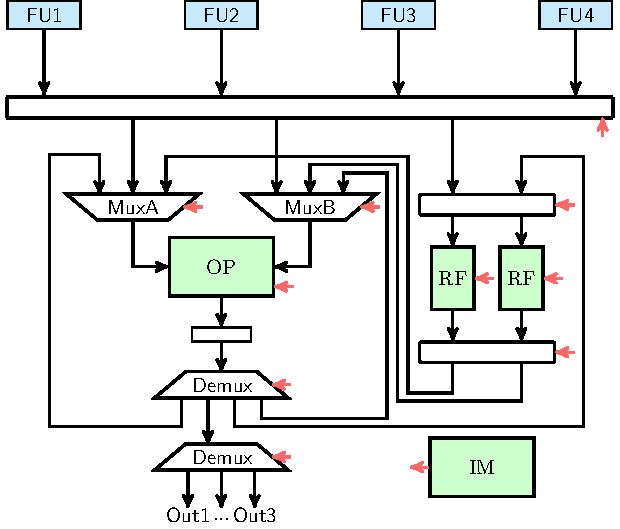
\includegraphics[width=.9\columnwidth,left]{images/functional_unit.pdf}
    \caption{\small Functional Unit template. The blocks at the top of the diagram represent other FUs that generate the inputs data. IM is the Instruction Memory, an internal memory where the FU stores the operation to perform. RFs are internal Register Files that the FU needs to reuse data and store inputs that needs to be used in the future. OP is the hardware unit actually performing the FU operation.}
\label{fig:FU_templ}
\end{figure}
